%!TEX root = main.tex
\newpage
\thispagestyle{plain}

\chapter{Plán práce na diplomovom projekte}

\section{Plán práce na diplomovom projekte I}

Prácu na diplomovom projekte I sme navrhli a naplánovali nasledovne:

\begin{table}[h]
\centering
\caption{Plán práce na diplomovom projekte I}
\begin{tabular}{|m{2.3cm}|m{12cm}|}
\hline
1-5.~týždeň semestra   & Analýza problematiky odporúčania v kontexte CQA systémov a súčasného výskumu v tejto oblasti. \\ \hline
6-7.~týždeň semestra   & Analýza dostupných dát na platforme Stack Exchange a možností verejného API platformy. \\ \hline
8-9.~týždeň semestra   & Vytvorenie predbežného návrh metódy riešenia problému a návrh metód overenia výsledkov. \\ \hline
10-12.~týždeň semestra & Spísanie správy diplomového projektu I v rátane analýzy a predbežného návrhu riešenia a overenia. \\ \hline
\end{tabular}
\end{table}

\textbf{Zhodnotenie}\\
Navrhnutý plán práce v rámci diplomového projektu I sa nám do veľkej miery podarilo dodržať. Časový sklz sa prejavil až
vo fáze návrhu metódy riešenia problému, čím sa posunulo spísanie správy až do 11. týždňa semestra.

\newpage
\section{Plán práce na diplomovom projekte II}

\begin{table}[h]
\centering
\caption{Plán práce na diplomovom projekte II}
\begin{tabular}{|m{2.3cm}|m{12cm}|}
\hline
1-2.~týždeň semestra   & -- Príprava databázy a aktualizačného modulu.
				\newline -- Vytvorenie modelov pre získavanie spätnej väzby od používateľov.
				\newline -- Prvotná dátová analýza.
				\\ \hline
3-4.~týždeň semestra   & -- Príprava rozhrania pre odoberanie informačných bulletinov.
				\newline -- Generovanie informačných bulletinov na základe prvotného modelu.
				\newline -- Nasadenie systému a otestovanie v reálnych podmienkach.
				\\ \hline
5-8.~týždeň semestra   & -- Získavanie používateľov informačného bulletinu.
				\newline -- Spracovanie dát, vytvorenie reálnych modelov používateľov a otázok, generovanie odporúčaní.
				\newline -- Príprava metód diverzifikácie odporúčaní.
				\newline -- Písanie diplomovej práce.
				\\ \hline
9-12.~týždeň semestra  & -- Overenie a vyhodnocovanie informačných bulletinov.
				\newline -- Nasadenie a porovnanie metód diverzifikácie.
				\newline -- Počiatočné overenie výsledkov.
				\newline -- V prípade neúspechu online experimentu, plánovanie offline expermientov.
				\\ \hline
\end{tabular}
\end{table}

\textbf{Zhodnotenie}\\
\textbf{TODO}

\section{Plán práce na diplomovom projekte III}

\textbf{TODO}

\begin{table}[h]
\centering
\caption{Plán práce na diplomovom projekte III}
\begin{tabular}{|m{2.3cm}|m{12cm}|}
\hline
1. mesiac & Pokračovanie v experimentoch, nasadzovanie systému na väčšom množstve dát. \\ \hline
2. mesiac & Analýza výsledkov experimentov, vyhodnotenie úspešnosti projektu. \\ \hline
3. mesiac & Dokončenie diplomovej práce.\\ \hline
\end{tabular}
\end{table}


\chapter{Technická dokumentácia systému}\label{tech-doc}

\section{Modul pre registráciu nových používateľov}

Tento modul predstavuje webovú aplikáciu určenú na registráciu nových používateľov systému StackLetter. Implementovaná je
v jazyku PHP 7.1 s použitím MVC/MVP webového frameworku Nette 2.4. Ďalej popisujeme niektoré dôležité komponenty tohto modulu.

\textbf{HomepagePresenter}\\
Táto trieda zabezpečuje hlavnú funkcionalitu stránky -- autentifikáciu a registráciu používateľov, ako aj manažment
používateľského konta. Autentifikácia používateľa sa vykonáva prostredníctvom Stack Exchange API s využitím protokolu OAuth 2.0.
Zabezpečuje tiež funkcionalitu kontaktného formuláru.

\textbf{SubscriptionPresenter}\\
Spolu s príslušnou modelovou triedou \textit{SubscriptionModel} implementuje možnosť odhlásenia sa z odoberania
informačného bulletinu, generovanie \textit{unsubscribe} odkazov pre jednotlivé informačné bulletiny, zbieranie spätnej
väzby po odhlásení sa z odoberania a možnosť opätovného prihlásenia sa.

\textbf{AsyncJobProcessor}\\
Táto trieda zabezpečuje asynchrónne spracovanie dlhotrvajúcich úloh. Vďaka asynchrónnemu spracovaniu týchto úloh ostáva
odozva používateľského rozhrania rýchla. Konkrétne vykonáva odoslanie uvítacieho e-mailu používateľovi po úspešnej
registrácii prostredníctvom služby SendGrid s využitím protokolu SMTP, a následné stiahnutie používateľského profilu
prostredníctvom Stack Exchange API.
Samotná webová aplikácia zadáva tejto komponente úlohy na asynchrónne spracovanie prostredníctvom Redis fronty.


\section{Modul pre generovanie a odosielanie informačných bulletinov}

\textbf{TODO}

\begin{figure}[H]\begin{center}
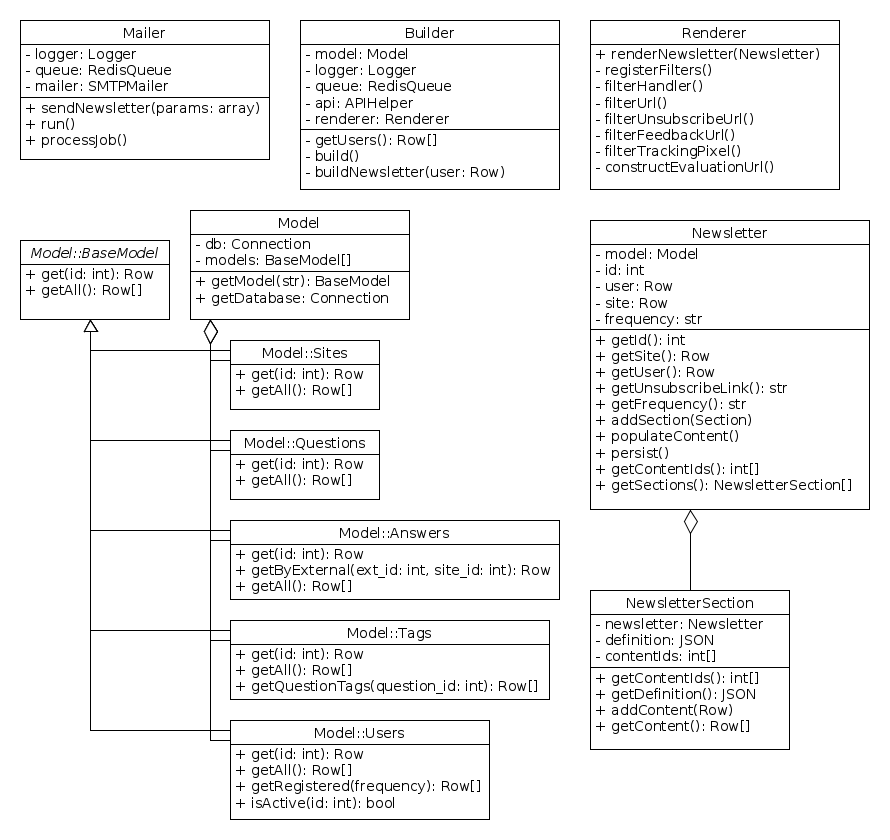
\includegraphics[scale=0.355]{mailer-schema}
\caption{Schéma modulu pre generovanie a odosielanie informačných bulletinov \label{fig:mailer-schema}}\end{center}
\end{figure}

\section{Modul pre spracovanie statickej zálohy databázy}

\textbf{TODO}

\section{Databázový model}
\begin{figure}[H]\begin{center}
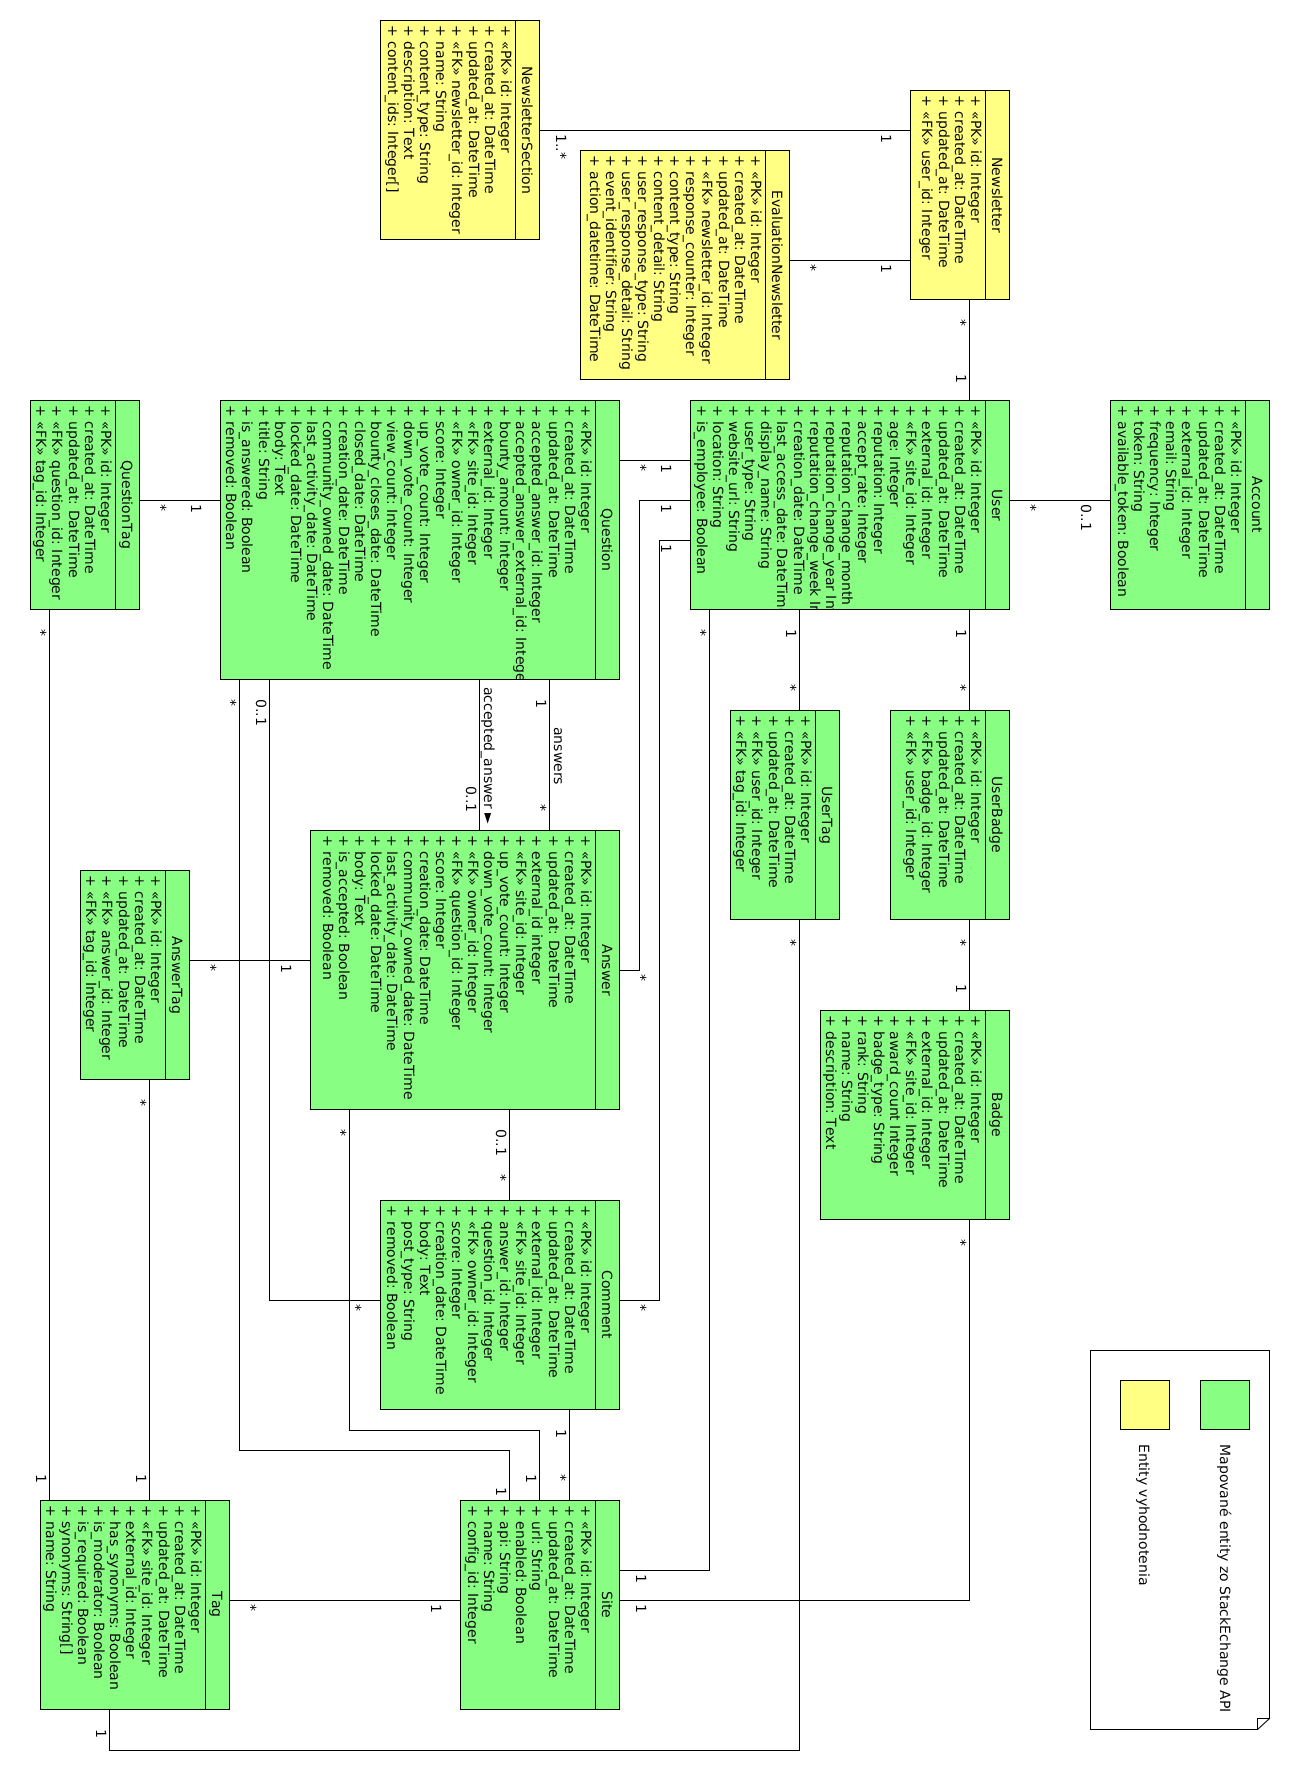
\includegraphics[scale=0.355]{db-model}
\caption{Databázový model systému StackLetter. Autor: Matúš Salát~\cite{Salat2018}. \label{fig:db-model}}\end{center}
\end{figure}

